
\subsubsection{Overview}

The methodology has four components: (1) checkpoint-level evaluation across the Pythia model family, (2) 13-gram contamination measurement using established decontamination tools, (3) capability detrending via out-of-distribution perplexity regression, and (4) Spearman correlation analysis between contamination and inflation residuals.

\subsubsection{Checkpoint-Gradient Methodology}

\textbf{Rationale.} Traditional contamination studies compare contaminated versus decontaminated models or use synthetic injection. Both approaches require either clean baseline models (which do not exist at scale) or artificial contamination (which may not reflect natural training dynamics). Checkpoints during training naturally vary in contamination exposure---early checkpoints have processed less of the training corpus, thus encountered less benchmark-overlapping content.

\textbf{Implementation.} The Pythia model family \citep{biderman2023pythia} trained on The Pile \citep{gao2020pile} provides:
\begin{itemize}
\item Six model sizes: 410M, 1B, 1.4B, 2.8B, 6.9B, 12B parameters
\item 154 checkpoints per model at documented training steps
\item Deterministic training order (same data sequence across all sizes)
\item Documented training corpus enabling ground-truth contamination measurement
\end{itemize}

\subsubsection{Contamination Measurement}

\textbf{N-gram overlap.} Following Brown et al. [2020], 13-gram overlap serves as the contamination metric. For each benchmark, the percentage of test items containing 13-gram sequences that appear in The Pile training corpus is computed.

\textbf{Cumulative exposure proxy.} For checkpoint-level analysis, cumulative contamination exposure is approximated as proportional to training progress---a checkpoint at step 100,000 has seen approximately 70\% of training data, thus approximately 70\% of contamination-relevant content.

\subsubsection{Capability Detrending}

\textbf{The confound.} Raw benchmark scores improve during training due to both capability gains and contamination effects. These must be separated to isolate contamination inflation.

\textbf{Detrending approach.} WikiText-103 perplexity serves as a contamination-independent capability measure. For each checkpoint:

$$\text{score}_{\text{expected}} = \alpha + \beta \cdot \log(1/\text{perplexity})$$

\textbf{Inflation residual.} The inflation residual is defined as:

$$\text{inflation}_i = \text{score}_i - \text{score}_{\text{expected},i}$$

Positive residuals indicate scores higher than capability would predict.

\begin{figure}[htbp]
\centering
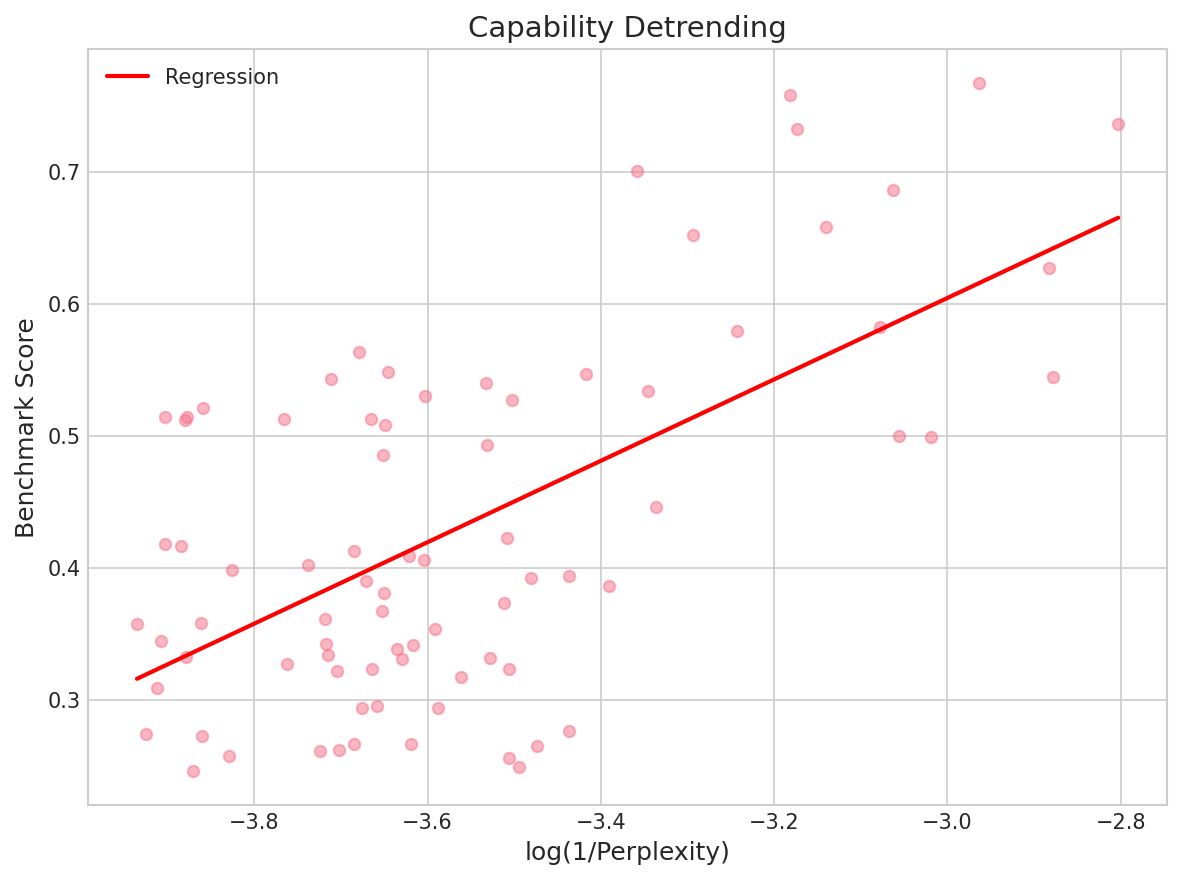
\includegraphics[width=\columnwidth]{figures/capability_detrending.png}
\caption{Capability Detrending}
\label{fig:capability_detrending}
\end{figure}

\textit{Figure 1: Capability detrending via WikiText-103 perplexity. Each point represents a checkpoint; the regression line represents expected score given capability. Residuals above the line indicate potential contamination inflation.}

\subsubsection{Correlation Analysis}

\textbf{Spearman correlation.} Spearman's rank correlation is computed between contamination percentage and inflation residual across all checkpoint-benchmark pairs. Statistical significance is assessed at p < 0.05.

\textbf{Success criteria:}
\begin{itemize}
\item Minimum threshold: r > 0.2 (weak-to-moderate correlation)
\item Primary target: r > 0.5 (strong correlation)
\end{itemize}

